\begin{frame}{Comparando métodos de estimação}
 \begin{itemize}
  \item Estimadores de Bayes~\textit{vs} EMV;
  \item Método dos momentos.
 \end{itemize}
\end{frame}

\begin{frame}{Bayes~\textit{vs} EMV}
Argumentos assintóticos:
  \begin{equation*}
   L(\theta) \approx \exp\left[-\frac{\left(\theta-\hat{\theta}\right)^2}{2V_n(\theta)/n} \right].
  \end{equation*}
 \begin{exemplo}[ Exemplo 7.6.11 em DeGroot]
    $\rs \sim \operatorname{Exponencial}(\theta)$, 
    \begin{itemize}
     \item   $\hat{\theta}_{\text{EMV}} = \left(\bar{X}_n\right)^{-1} \implies E[\hat{\theta}_{\text{EMV}}] = \theta$ e $\vr[\hat{\theta}_{\text{EMV}}] = \theta^2$.
  Pelo método Delta, temos $\hat{\theta}_{\text{EMV}} \approx \operatorname{Normal}(\theta, \theta^2/n)$;
    \item Se escolhemos uma priori gama para $\theta$ com hiperparâmetros $\alpha > 0$ e $\beta > 0$,    temos $E_{\theta \mid \boldsymbol{x}}[\theta] = (\alpha + n)/(\beta + S_n)$ e $\vr_{\theta \mid \boldsymbol{x}}(\theta) = (\alpha + n)/ (\beta + S_n)^2$.
    Fazendo $\alpha, \beta \ll n$, temos um argumento análogo para o estimador de Bayes.
    \end{itemize}  
 \end{exemplo}
\end{frame}


\begin{frame}{EMV para taxa de uma exponencial (DG ex. 7.6.11)}
\begin{figure}[!ht]
\label{fig:mle_exponential_deltaMethod}
\begin{center}
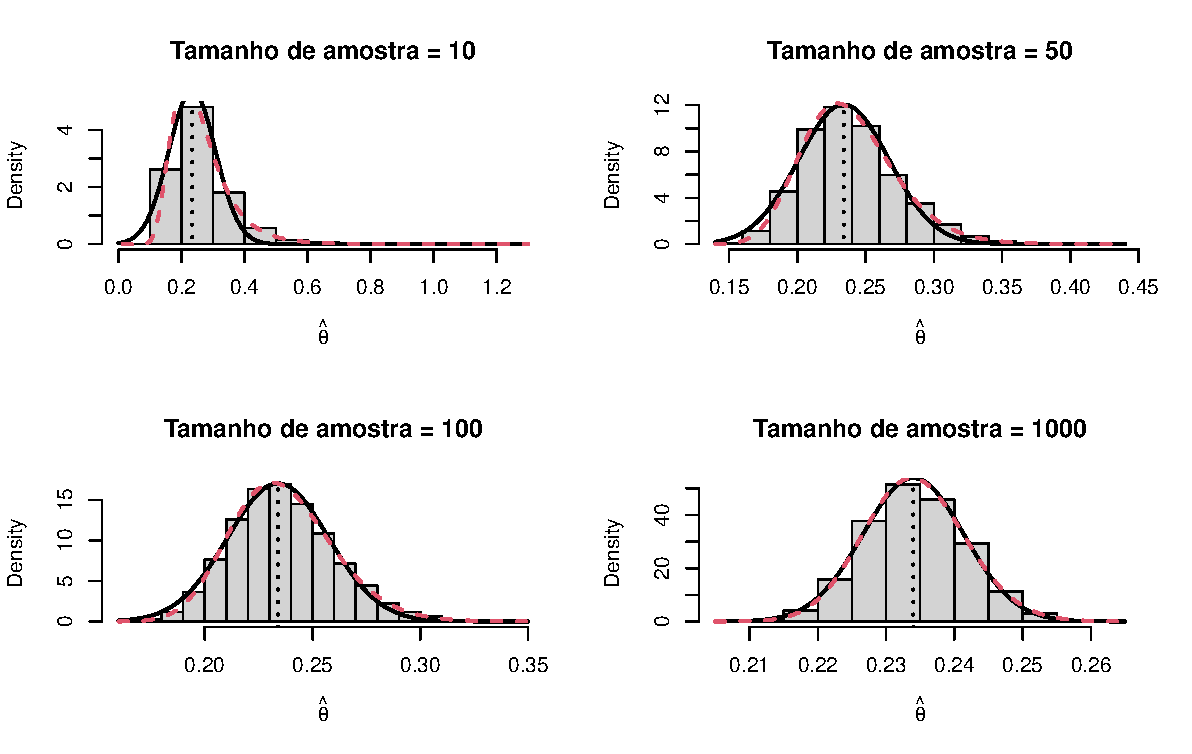
\includegraphics[scale=0.6]{figures/exponential_mle_deltaMethod.pdf} 
\end{center} 
\end{figure} 
\end{frame}

\begin{frame}{Inferência para uma Uniforme em $(0, \theta)$}
\begin{exemplo}[Exemplo 7.6.14 em DeGroot]
$\rs \sim \operatorname{Uniforme}(0, \theta)$.
Definindo $Y = \max(\rs)$ temos 
\[ g_n(y \mid \theta) = n\frac{y^{n-1}}{\theta^n}. \]
Como já discutido, temos $\hat{\theta}_{\text{EMV}} = \max(\rsd) = y_n$ e portanto
\begin{itemize}
 \item $E[\hat{\theta}_{\text{EMV}}] = \frac{n}{n + 1}\theta$;
 \item $\vr(\hat{\theta}_{\text{EMV}}) =  \frac{n}{(n + 1)^2(n+2)}\theta^2$.
\end{itemize}
Do lado bayesiano, vamos obter a posteriori (com uma priori imprópria):
  \begin{equation}
  \label{eq:uniform_reference_posterior}
    \xi(\theta \mid \boldsymbol{x})=
 \begin{cases}
     \frac{(n-1)y_n^{n-1}}{\theta^n}, y_n < \theta,\\
     0,\:\text{caso contrário}.
\end{cases}
 \end{equation}
Isto nos leva a
\begin{itemize}
 \item $E[\hat{\theta}_{\text{Bayes}}] = \frac{n-1}{n-2}y_n$;
 \item $\vr(\hat{\theta}_{\text{Bayes}}) =  \frac{n-1}{(n - 2)^2(n-3)}y_n^2$.
\end{itemize}
\end{exemplo}
\end{frame}

\begin{frame}{Método dos momentos (MM)}
 Algumas vezes, obter o EMV ou o estimador de Bayes envolve dificuldades numéricas (ex. estimar os parâmetros de uma distribuição Gama).
 Nestas situações, podemos encontrar um estimador para os parâmetros que relacione os momentos empíricos com os téoricos.
 
 \begin{defn}[Método dos momentos]
 \label{def:method_of_moments}
  Suponha que $\rs$ formam uma amostra aleatória com distribuição conjunta $f_n(\rs \mid \theta)$, $\theta \in \Omega \subseteq \mathbb{R}^k$ e que o $k$-ésimo momento existe.
  Defina $\mu_j(\theta) = E[X_1^j \mid \theta]$ e suponha que $\mu : \Omega \to  \mathbb{R}^k$ é biúnivoca, de modo que sua inversa é 
  \[ \theta = M(\mu_1(\theta), \ldots, \mu_k(\theta)).\]
 Dados os~\textit{momentos amostrais} $m_j := \frac{1}{n} \sum_{i=1}^n X_i^j$, $j = 1, \ldots, k$, o~\textbf{estimador de momentos} (EMM) de $\theta$ é 
 \[ \hat{\theta}_{\text{EMM}} = M(m_1, \ldots, m_k). \]
 \end{defn}
\end{frame}

\begin{frame}{Exemplo}
\begin{exemplo}
$\rs \sim \operatorname{Gama}(\alpha, \beta)$, com $\alpha >0$ e $\beta>0$ desconhecidos.
Para começar,
\begin{itemize}
 \item $\mu_1(\theta) = \alpha/\beta$;
 \item $\mu_2(\theta) = (\alpha + 1)\alpha/\beta^2$.
\end{itemize}
Agora equacionamos com os momentos amostrais (``empíricos''):
$\mu_1(\theta) = \bar{x}_n$ e $\mu_2(\theta) = \frac{1}{n}\sum_{i=1}^n x_i^2$ para obter
\begin{itemize}
 \item $\hat{\alpha} = \frac{(\bar{x}_n)^2}{\frac{1}{n}\sum_{i=1}^n x_i^2 - (\bar{x}_n)^2} = \frac{(\bar{x}_n)^2}{\bar{s}^2}$ ;
 \item $\hat{\beta} = \frac{\bar{x}_n}{\frac{1}{n}\sum_{i=1}^n x_i^2 - (\bar{x}_n)^2} = \frac{\bar{x}_n}{\bar{s}^2}$.
\end{itemize}
\end{exemplo}
  \begin{obs}
  O método dos momentos também pode ser usado para obter chutes iniciais para procedimentos numéricos nos métodos mais avançados (EMV, Bayes).
 \end{obs}
\end{frame}

\begin{frame}{Consistência do EMM}
 \begin{theo}[Consistência do EMM]
 \label{thm:MME_consistency}
    Suponha que $\rs$ formam uma amostra aleatória com distribuição comjunta $f_n(\rs \mid \theta)$, $\theta \in \Omega \subseteq \mathbb{R}^k$ e que o $k$-ésimo momento existe.
    Mais uma vez, suponha que a inversa $M$ existe e é contínua.
    Então o EMM é consistente para $\theta$.
 \end{theo}
\textbf{Prova}: Pela LGN, $m_i \xrightarrow{\text{p}}  \mu_i(\theta)$.
Assumindo que $M$ é contínua, temos que $M(m_1, \ldots, m_k) \xrightarrow{\text{p}} M(\mu_1(\theta), \ldots, \mu_k(\theta)) = \theta$  (DeGroot, Teorema 6.2.5).
\end{frame}

\begin{frame}{O que aprendemos?}
\begin{itemize}
  \item[\faLightbulbO] EMV~\textit{vs} Bayes;
 
   ``Em várias situações, à medida que $n \to \infty$, os estimadores 'convergem' ''
  
  \item[\faLightbulbO] Nem sempre EMV $\approx$ Bayes;
 
   ``Verossimilhanças discontínuas e/ou pequenos tamanhos de amostra''
   
  \item[\faLightbulbO] Método dos momentos (MM);
  
  ``Quando os momentos são funções inversíveis dos parâmetros, podemos obter estimadores em função dos momentos amostrais''
  
    \item[\faLightbulbO] Consistência do MM;
  
  ``Sob condições brandas de regularidade, o EMM converge para valor verdadeiro à medida que $n \to \infty$''
  
    \item[\faLightbulbO] Limitações do MM;
  
  ``Raras as situações em que tudo se alinha de modo que o EMM exista em forma fechada''
  
  \end{itemize}
 \end{frame}

\begin{frame}{Leitura recomendada}
\begin{itemize}
 \item[\faBook] DeGroot seção 7.6;
 \item[\faBook] $^\ast$ Schervish (1995), capítulo 7.
 \item[\faForward] Próxima aula: DeGroot, seções 7.7 e 7.8;
 \item {\large\textbf{Exercícios recomendados}}
 \begin{itemize}
  \item[\faBookmark] DeGroot, seção 7.6: exercícios 20, 22 e 23. 
%   \begin{itemize}
%    \item Seção 7.5: exercícios  1, 4, 9 e 10;
%    \item Seção 7.6: exercícios 3, 5, 11 e 20.
%   \end{itemize}   
  \end{itemize}
 \end{itemize} 
\end{frame}
